\subsubsection{Presencia de la resistencia $R_4$}
Se nos pidi\'o analizar la influencia de la resistencia $R_4$ en el circuito de configuraci\'on inversora.
En las expresiones de $V_{out}/V_{in}$ y $Z_{in}$ obtenidas para este circuito se observa que
esta resistencia no influye. Por lo tanto, variando dicho valor, la respuesta en frecuencia y la impedancia
de entrada al circuito seguir\'a siendo la misma.

\subsubsection{Ausencia de la resistencia $R_3$}

Para el caso del circuito no inversor, si $R_3$ vale cero, la impedancia de entrada valdr\'a lo mismo 
que $R_3$ en el c\'alculo te\'orico. No ocurre lo mismo para el circuito inversor. En este \'ultimo, 
la impedancia de entrada no depende de $R_3$, por lo que el valor de dicha impedancia no cambiar\'a
al anular $R_3$.

Al observar lo que ocurre con $V_{out}/V_{in}$, se puede ver que anulando $R_3$, disminuyela ganancia del circuito inversor, mientras que aumenta en el caso del no inversor.

\subsubsection{Selecci\'on de amplificador operacional para altas frecuencias}
Según el análisis realizado no sería conveniente emplear el lm324 para una se\~nal cuya 
frecuencia oscile entre 0.3Mhz y 2Mhz. En este punto se puede observar que la ganancia 
en tensión es casi nula, por lo que el amplificador operacional dificilmente podrá ser usado 
para amplificar. Esto se puede observar en el siguiente gráfico, extraído de la wwb de Texas 
Instruments.

\begin{figure}[H] %!ht
	\centering
	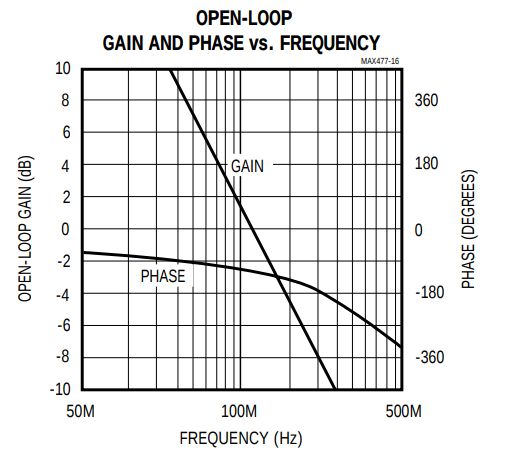
\includegraphics[width=10cm,height=10cm,keepaspectratio]{../EJ1/00GRAFICOS/imagenes/EJ1_avol_max477.png}
	\caption{Ganancia a lazo abiero del LM324 en funci\'on de la frecuencia.}
	\label{i1}
\end{figure}

Por otro lado también se debe tener en cuenta el efecto del slew rate. Con una tensión pico a pico de 1V y variando la frecuencia en el rango mencionado arriba y además suponiendo ganancia unitaria tendríamos un coeficiente de slew rate que oscila entre 1.8 y 12.56 volts por microsegundo. Esto supera ampliamente al propio coeficiente máximo extraído de la datasheet del componente. Este úlltimo vale 0.5 volt por microsegundo. Consecuentemente, la se\~nal de salida se verá gravemente distorsionada a causa de este efecto, aún en el mejor de los casos de amplificación.

Por otro lado este amplificador operacional tiene un coeficiente de slew rate de 1100 volts por microsegundo, cuatro veces superior en orden de magnitud al del LM324. Cabe destacar que este amplificador está pensado para frecuencias muy superiores al rango solicitado, por lo que su aplicación en dicho rango seguramente será poco eficiente en términos de costo  beneficio.

Otra opción un tanto más lógica en terminos de costos sería la serie OPA141 de Texas Instruments. Estos amplificadores están dise\~nados para operar en frecuencias del orden de los 10MHz. En cuanto al slew rate, el coeficiente característico de esta familia es de 20 volt por microsgundo (lo que implica que las se\~nales mencionadas en el apartado anterior entran en el rango de no distorsión). Respecto a la ganancia  del operacional, en el siguiente gráfico se puede veirificar que la ganancia a lazo cerrado es superior a la unitaria, por lo que puede ser configurable para que valga uno.

\begin{figure}[H] %!ht
	\centering
	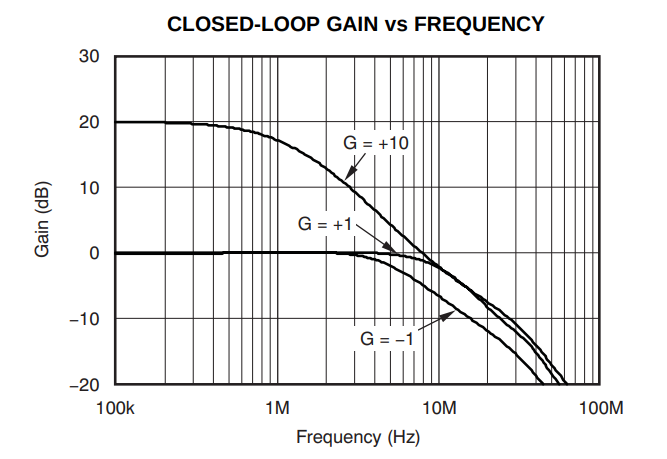
\includegraphics[width=10cm,height=10cm,keepaspectratio]{../EJ1/00GRAFICOS/imagenes/EJ1_avcl_OPA141.png}
	\caption{Ganancia a lazo cerrado del OPA141}
	\label{i2}
\end{figure}

Por último, psteodemos mencionar al modelo TSX920 de ST. Al igual que el anterior este circuito integrado está dise\~nado para trabajar a frecuencias del orden de los 10MHz. En este caso el slew rate está afectado por el signo de la pendiente de la se\~nal, valiendo su coeficiente 17.7 y 19.6 volt por microsegundo con pendiente positiva y negativa respectivamente. Desde este punto de vista es apto para la aplicación solicitada.  Por otro lado, abajo se puede observar que la ganancia a lazo abierto es suficiente para obtener gananicia unitaria, en las frecuencias de trabajo del amplificador.

\begin{figure}[H] %!ht
	\centering
	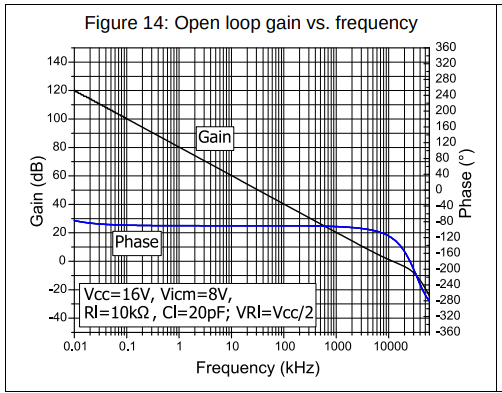
\includegraphics[width=10cm,height=10cm,keepaspectratio]{../EJ1/00GRAFICOS/imagenes/EJ1_avol_tsx920.png}
	\caption{Ganancia a lazo cerrado del TXS920.}
	\label{i2}
\end{figure}